\section{Vehicle Actuated Programming in Vissim}
\label{vap}
VAP is an optional module for Vissim which enables direct programming of signal controllers. VAP is a simple, label-based (goto) language. The main feature is access to a library of functions, which manipulate the state of the signal controller. 

With VAP there is a graphical program, VISVAP, that allows the user to design a flowchart description of the controller logic, rather than writing it in VAP, as VISVAP can compile the flowchart into VAP. Figure \ref{fig:visvap_example} shows an example of a simple logic to control the lights at the ring 3 / Herlev Sygehus intersection.

\begin{figure}[!ht]
\begin{center}
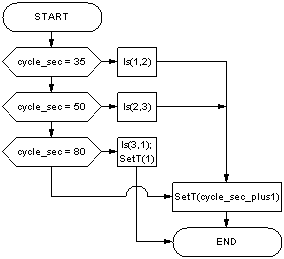
\includegraphics[scale=0.5]{visvap_example_herlev-sygehus.png} 
\end{center}
\caption{VISVAP flowchart description of simple fixed-time logic for Herlev Sygehus / ring 3}
\label{fig:visvap_example}
\end{figure}

The VAP program is called once for every simulation second. The starting label is START and the program proceeds as indicated by the arrows until the END label has been reached. Diamond boxes are logical tests where the right-going arrow indicates TRUE and down-going indicates FALSE. Square boxes contain expressions, in this case we use \verb|Is(<stage_from>,<stage_to>)| to switch between stages, when a certain portion of the current cycle time has passed. Below is the VAP code, which corresponds to the flowchart:

\begin{verbatim}
/* EXPRESSIONS */ 
            cycle_sec := T;
            cycle_sec_plus1 := cycle_sec + 1;

/* MAIN PROGRAM */ 

S00Z001:    IF cycle_sec = 35 THEN
S01Z001:      Is(1,2)
            ELSE
S00Z002:      IF cycle_sec = 50 THEN
S01Z002:        Is(2,3)
              ELSE
S00Z003:        IF cycle_sec = 80 THEN
S01Z003:          Is(3,1); SetT(1);
                  GOTO PROG_ENDE
                END
              END
            END;
S02Z004:    SetT(cycle_sec_plus1)
PROG_ENDE:    .
\end{verbatim}

VAP is unsuited for complex controller logic, such as ones involving predictions and optimization by iteration. This is due to the fact that VAP only has support for basic programming language constructs and the label-based nature of the language, which is detrimental to larger code bases see eg. the statement by Dijkstra \cite{nogoto}. As an example the above VAP code could be simplified into:

\begin{verbatim}
function UpdateController(cycle_second){
   switch(cycle_second){
   case 35: Interstage(1,2)
   case 50: Interstage(2,3)
   case 80: Interstage(3,1); Set_cycle_second(1); return
   case else:  /* do nothing */
   }
   Set_cycle_second(cycle_second + 1) /* update time */
}
\end{verbatim}

VAP is suitable, however, for implementation of DOGS due to its simple decision system as described in section \ref{dogs}. In this section I will describe how the DOGS logic was implementated in VAP.

\subsection*{Interstage Definitions - PUA}
Before we move on to DOGS in VAP it is fundamental to explain the \verb|Interstage| (abbr. \verb|Is|) concept. Interstage definitions are mandatory in Vissim whenever a VAP program is to control a signal.

An interstage is basically the lighting scheme to be used during stage transition. Usually, when switching from stage A to B the lights of A switch to amber and then red while B switch from red to red and amber and then green.

The amber light of A is a warning that a transition is in progress, the intersection should be cleared and no more entries should be made. To ensure right-of-way consistency during the transition, B will stay red until the moment A switches from amber to red. For all intersections discussed in this project, the amber period is 4 seconds.

The red and amber period of B indicates that attentive entry into the intersection is permitted. The red and amber period is 2 seconds for all intersections.

Thus a total stage transition will last 6 seconds. In Figure \ref{fig:lost_time_example} is an example of the interstage lost times for various number of stages and cycle times. Some stages - eg. a through, left and rightgoing stage followed by a left-only stage - will be \textit{compatible} ie. there is no pause during the transition thus the table is pessimistic. However it clearly shows that there is a tradeoff between lost time and cycle time - especially in complex, multistaged intersections.

\begin{figure}[!ht]
\begin{center}
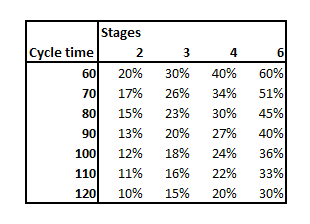
\includegraphics[scale=0.6]{interstage_lost_time.png} 
\end{center}
\caption{Interstage lost time in percent of cycle time for some combinations of cycle time and number of incompatible stages}
\label{fig:lost_time_example}
\end{figure}

In the above flowchart and code examples we start an interstage whenever we wish to move to the next stage.

The interstages are defined in Vissim by .PUA files. Below is an example of such a definition for Herlev Bygade. This intersection has two stages; stage A allowing traffic in either direction of the arterial and stage B for turn-ins from the minor road. 

\begin{verbatim}
$SIGNAL_GROUPS
A   1
B   2

$STAGES
Stage_1   A
red       B
Stage_2   B
red       A

$STARTING_STAGE
Stage_1

$INTERSTAGE1
Length [s]	 :   6
From Stage	 :   1
To Stage	   :   2
$    redend   grend
A    -127     0
B       4     127

$INTERSTAGE2
Length [s]	: 6
From Stage	: 2
To Stage	: 1
$    redend   grend
B    -127     0
A       4     127
$END
\end{verbatim}

In section \$STAGES it is defined that stage A should be green while B should is red and vice versa (they are not compatible). Here A and B refers to a space-separated list of signal groups from the \$SIGNAL\_GROUPS section.

For the interstage definitions, in INTERSTAGE1, we have redend for A to be -127, which means that A is green before the interstage, and grend (green end) is 0 meaning it should be red when the interstage has completed. For stage B, which is red before the interstage is run due to the \$STAGES definition, the redend (=green start) occurs 6 seconds into the interstage and grend set to 127 means that B should remain green after the interstage.

It is always up to the interstage designer to ensure that no right-of-way conflicts are present in the stage definitions. PTV supplies a support tool, which solves this issue, called CROSSIG. CROSSIG is capable of generating .PUA files; in this project CROSSIG was not available, however, and they were generated automatically from the signal plans, which are listed in appendix \ref{app:signalplans}.

\subsection*{Interstage rules}
The signal plans, for which interstage definitions are to be built, are formatted so that each named signal group (head) has a row with $C$-cells, where $C$ is the cycle time. Each cell can be amber, green, yellow or red. Thus a complete signal timing plan is visually represented as one or more such rows in a stack.

In order to generate the interstage definitions (.PUA files in Vissim) it is necessary with a definition of an interstage itself. A stage is said to \textit{run} while the signal groups of the stage is settled in the green state. We define that when a stage is running an interstage cannot run and vice versa. Thus every cycle second must specify the current stage or interstage.

An interstage runs whenever one or more signal groups receive new colors until the changes of color have settled. This could for instance be the green end for group A, which is the start of an interstage cycle second the group begins to show yellow, until the perpendicular group, B, has settled its green light, which could include amber time. In the sample .PUA file above we see the implementation of this exact scenario: A ends its green time in interstage second 1 and B begins its amber-green time 4 seconds later, while group A is showing yellow. Group B shows amber for 2 seconds and thus the total length of the interstage is 6 seconds. 

It is important to note that, while stages must have a temporal extend to make sense, interstages may have zero length. Such interstages occur when light switch directly from red to green (respecting safety) and from green to red without the ordinary amber and yellow time respectively. Amber and yellow times are defined in the Vissim network file (.INP) and cannot be controller in the interstage definitions. Amber and yellow time is automatically appended by Vissim to the green- and red end times when the VAP controller runs an interstage.

A safety period, where all heads are red, is sometimes introduced in order to allow the intersection to be cleared. This can be modelled either as a stage with no green signal groups or included into the interstage definition by prolonging red end times and interstage length by the length of the safety period. The latter solution is preferred since it is directly supported in the PUA format and also avoids the introduction of an all-red stage and a number of extra interstages to and from the all-red stage.

\subsection{DOGS}
As VAP does not permit the writing of a program, which supervise all signal controllers at the same time, it was necessary to dedicate a signal controller as the master controller. To fully separate the master/slave concept it was chosen to install a virtual signal controller, whose only purpose is to run the DOGS program.

The master controller, which for the purpose of offset has a virtual location on Herlev Hovedgade, runs the DOGS program and determines the current level by inspecting the northern- and southern detectors according to the specification outlined in section \ref{dogs}. In addition this controller also runs the master clock and the current DOGS level and master cycle second is sent to all slave controllers every cycle second.

The slave signal controller - even the one on Herlev Hovedgade - must listen for communication from the master controller and set the green time of the various stages according to the current dogs level and cycle second as received from the master.

Both master and slave VAP controllers are generated automatically using a script, which takes parameters such as, for the master, the area-specific detectors and activation / level-up / level-down bounds and, for the slave, offset value(s), signal program etc.

\subsection*{Master}
Relevant to master controllers we need to know the northern and southern detector names as these are used to determine if DOGS is enabled or turned off. Once DOGS is enabled another set of detectors (possibly overlapping) are measured upon to determine the appropriate level of DOGS. Note that, depending on threshold values, DOGS may be \textit{enabled} but not perform adjustments to the base-program - this is by design.

These threshold values are also parameters which is fed into the generator routine (see section \ref{dogs} for a description). 
Due to variations between the traffic, which TTS used to tune the threshold values, and the traffic which is observed in the simulation, it was decided to manually retune the vehicle count thresholds while keeping the thresholds for occupancy. 
Along with the detector data described in section \ref{detector_data} TTS supplied the selected DOGS levels in the same period. By a manual, iterative process the levels selected by DOGS in the simulator was fitted to the levels of the detector data set during the morning period. The main fixpoints used was the maximum and the average levels chosen.

DOGS accumulate detections over a cycle - which is of variable length - and compare to the threshold values. Occupancy is a the percentage of time of which the detector was enabled ie. a vehicle passed over or was in queue over the detector and thus the detection period can be chosen freely. The amount of vehicles which passed over (the 2nd component for threshold matching) is in total numbers and consequently when the cycle time increase so does the number of detected vehicles. TTS informs me that no adjustment - except for the standard exponential smoothening - is performed when comparing detector vehicle count values with the thresholds. I decided to correct this in the VAP code by assuming the counting thresholds matched a 80 seconds cycle and then scale the detected count to this level by using the actual cycle time (which is usually higher, when DOGS is enabled).

When DOGS is active the level is adjusted at most by one for each cycle. Thus when the level is high it will take longer to change between levels and the measuring periods are longer, resulting in more accurate measurements, but less responsiveness.

\subsection*{Slave}
The purpose of slave controllers is to obey the cycle second and DOGS level instructions from the master controller.

The first step for a slave is to calculate the local cycle second, which due to controller offset will usually differ from the master cycle second. An exception is the slave controller, which controls the intersection in which the master controller is physically positioned - the distance between them is 0 and likewise the offset.

Consider stage A which is active while the master controller lowers the DOGS level by 1. In this case the end time is lowered if stage A receives priority from DOGS and it may happen that the end time for stage A is now lower then the current cycle second. Stage A will then have received more green time than it was supposed to and the slave will immediately make the transition from stage A to the next stage, B. In case B is not the stage which was supposed to be active (a rare case - stage B is short indeed) we allow stage A to carry over to the next cycle as we can only make stage transitions between subsequent stages - not in arbitrary order.

\subsection*{Bus Priorities}
Three intersections in the Glostrup area - Fabriksparken, Gammel Landevej and Kindebjergvej - operate with bus priority on the arterial direction. 

If a bus arrives from north or south during the stage which belongs to the arterial green time of up to 10 seconds is distributed from the minor road stage to this stage. The effect is that buses might just make it across before the next stage is started rather than being cut off. In the next cycle the main stage is shortened by the same amount of time and the minor stage is lengthened accordingly.

This is implemented by associating detectors for north- and southgoing buses for each of these intersections. The autogenerated VAP code will then check for bus detections in each cycle second and perform bus prioritization if:

\begin{enumerate}
\item The main stage is the currently active stage
\item The signal controller is not currently performing a bus prioritization
\item The signal controller is not currently compensating the minor road stage due to prioritization in the previous cycle
\end{enumerate}

When bus prioritization is activated under these conditions the stage end times will be adjusted as mentioned and the next cycle (compensation) will perform likewise adjustments albeit inversed.

In case that a bus arrives and activates bus prioritization but make it across the intersection before the green time for the stage has been extended, bus prioritization is cancelled.